\documentclass[oneside,12pt,a4paper]{book}

\usepackage[T1]{fontenc} %normes d'encodage
\usepackage[utf8]{inputenc} %normes d'encodage
\usepackage[inner=25mm,outer=25mm,top=30mm,bottom=20mm,headheight=13.6pt]{geometry} %marges
\usepackage{lmodern} %correction d'affichage
\usepackage{graphicx} %insertion d'images
\usepackage{csquotes} %guillemets français
\usepackage{sectsty} %modifier l'apparence des titres
\usepackage{fancyhdr} %en tête et pieds de page personnalisables
\usepackage{etoolbox} %idem
\usepackage{color} %gestion des couleurs
\usepackage{setspace} %interligne
\usepackage{natbib} %pour pouvoir ne citer que l'année
\usepackage[french]{babel} %langue française
\usepackage{chngcntr} %compteurs modifiables
\usepackage{amsmath} %package maths
\usepackage{amssymb} %package maths
\usepackage[lite]{mtpro2} %package maths
\usepackage{url} %gestion des liens hypertextes
\usepackage{blindtext} %génération de texte aléatoire : \Blindtext
\usepackage{tikz} %dessin (pour la page de garde)

\counterwithout{figure}{chapter} %permet un numérotage des figures indépendant des chapitres
\frenchspacing %adaptation normes françaises
\FrenchFootnotes %adaptation normes françaises
\onehalfspacing %Interligne 1,5
\setcounter{secnumdepth}{4} %chapitrage à 4 niveaux (ex: 1.2.2.3. Lorem Ipsum)
\setcounter{tocdepth}{4} % chapitrage à 4 niveaux dans le sommaire

%%%%%%%%%%%%%%%%%%%%%%%%%%%%%%%%%%%%%%%%%%%%%%%%%%%%%%%%%%%%%%%
%%%%%%%%%%%%%%%%%%% Chapitrage personnalisé %%%%%%%%%%%%%%%%%%%
% Inspiré du thème Bredele

\makeatletter
\def\thickhrulefill{\leavevmode \leaders \hrule height 1ex \hfill \kern \z@}
\def\@makechapterhead#1{%
  \vspace*{-30\p@}%
  {\parindent \z@ \raggedleft \reset@font
            \scshape \@chapapp{} \thechapter
        \par\nobreak
        \interlinepenalty\@M
    \Huge \bfseries #1\par\nobreak
    %\vspace*{1\p@}%
    \hrulefill
    \par\nobreak
    \vskip 50\p@
  }}
\def\@makeschapterhead#1{%
 \vspace*{-50\p@}%
  {\parindent \z@ \raggedleft \reset@font
            \scshape \vphantom{\thechapter}
        \par\nobreak
        \interlinepenalty\@M
    \Huge \bfseries #1 \par\nobreak
    %\vspace*{1\p@}%
    \hrulefill
    \par\nobreak
    \vskip 30\p@
  }}

\fancyhf{} 

\appto\mainmatter{\pagestyle{fancy}
\renewcommand{\sectionmark}[1]{\markright{\textit{\thesection.\ #1}}}
\renewcommand{\chaptermark}[1]{\markboth{\textit{#1}}{}}
\fancyhead[L,R]{\small\thepage}
    \fancyhead[R]{\small\rightmark}
    \fancyhead[L]{\small \leftmark}
    \fancyfoot[C]{\thepage}
}
%%%%%%%%%%%%%%%%%%%%%%%%%%%%%%%%%%%%%%%%%%%%%%%%%%%%%%%%%%%%%
%%%%%%%%%%%%%%%%%%%%%%%%%%%%%%%%%%%%%%%%%%%%%%%%%%%%%%%%%%%%%


\title{Rapport de projet J2E}

\begin{document}


%%%%%%%%%%%%%%%%%%%%%%%%%%%%%%%%%%%%%%%%%%%%%%%%%%%%%%%%%%%%
%%%%%%%%%%%%%%%%%% Page de garde %%%%%%%%%%%%%%%%%%%%%%%%%%%
\thispagestyle{empty}
\begin{tikzpicture}[remember picture, overlay, shift=(current page.south)]
  \draw[gray] (current page.north west) rectangle (-4.5,0) ;
  \shade[top color=white , bottom color=gray] (current page.north west) rectangle (-4.5,0) ;
\end{tikzpicture}
\begin{tikzpicture}[remember picture, overlay, shift=(current page.north west)]
  \node[inner sep=0pt] (ensias) at (3,-4)
    {\includegraphics[width=.225\textwidth]{Ensias.png}};
  \node[inner sep=0pt] (chatvideo) at (3,-26)
    {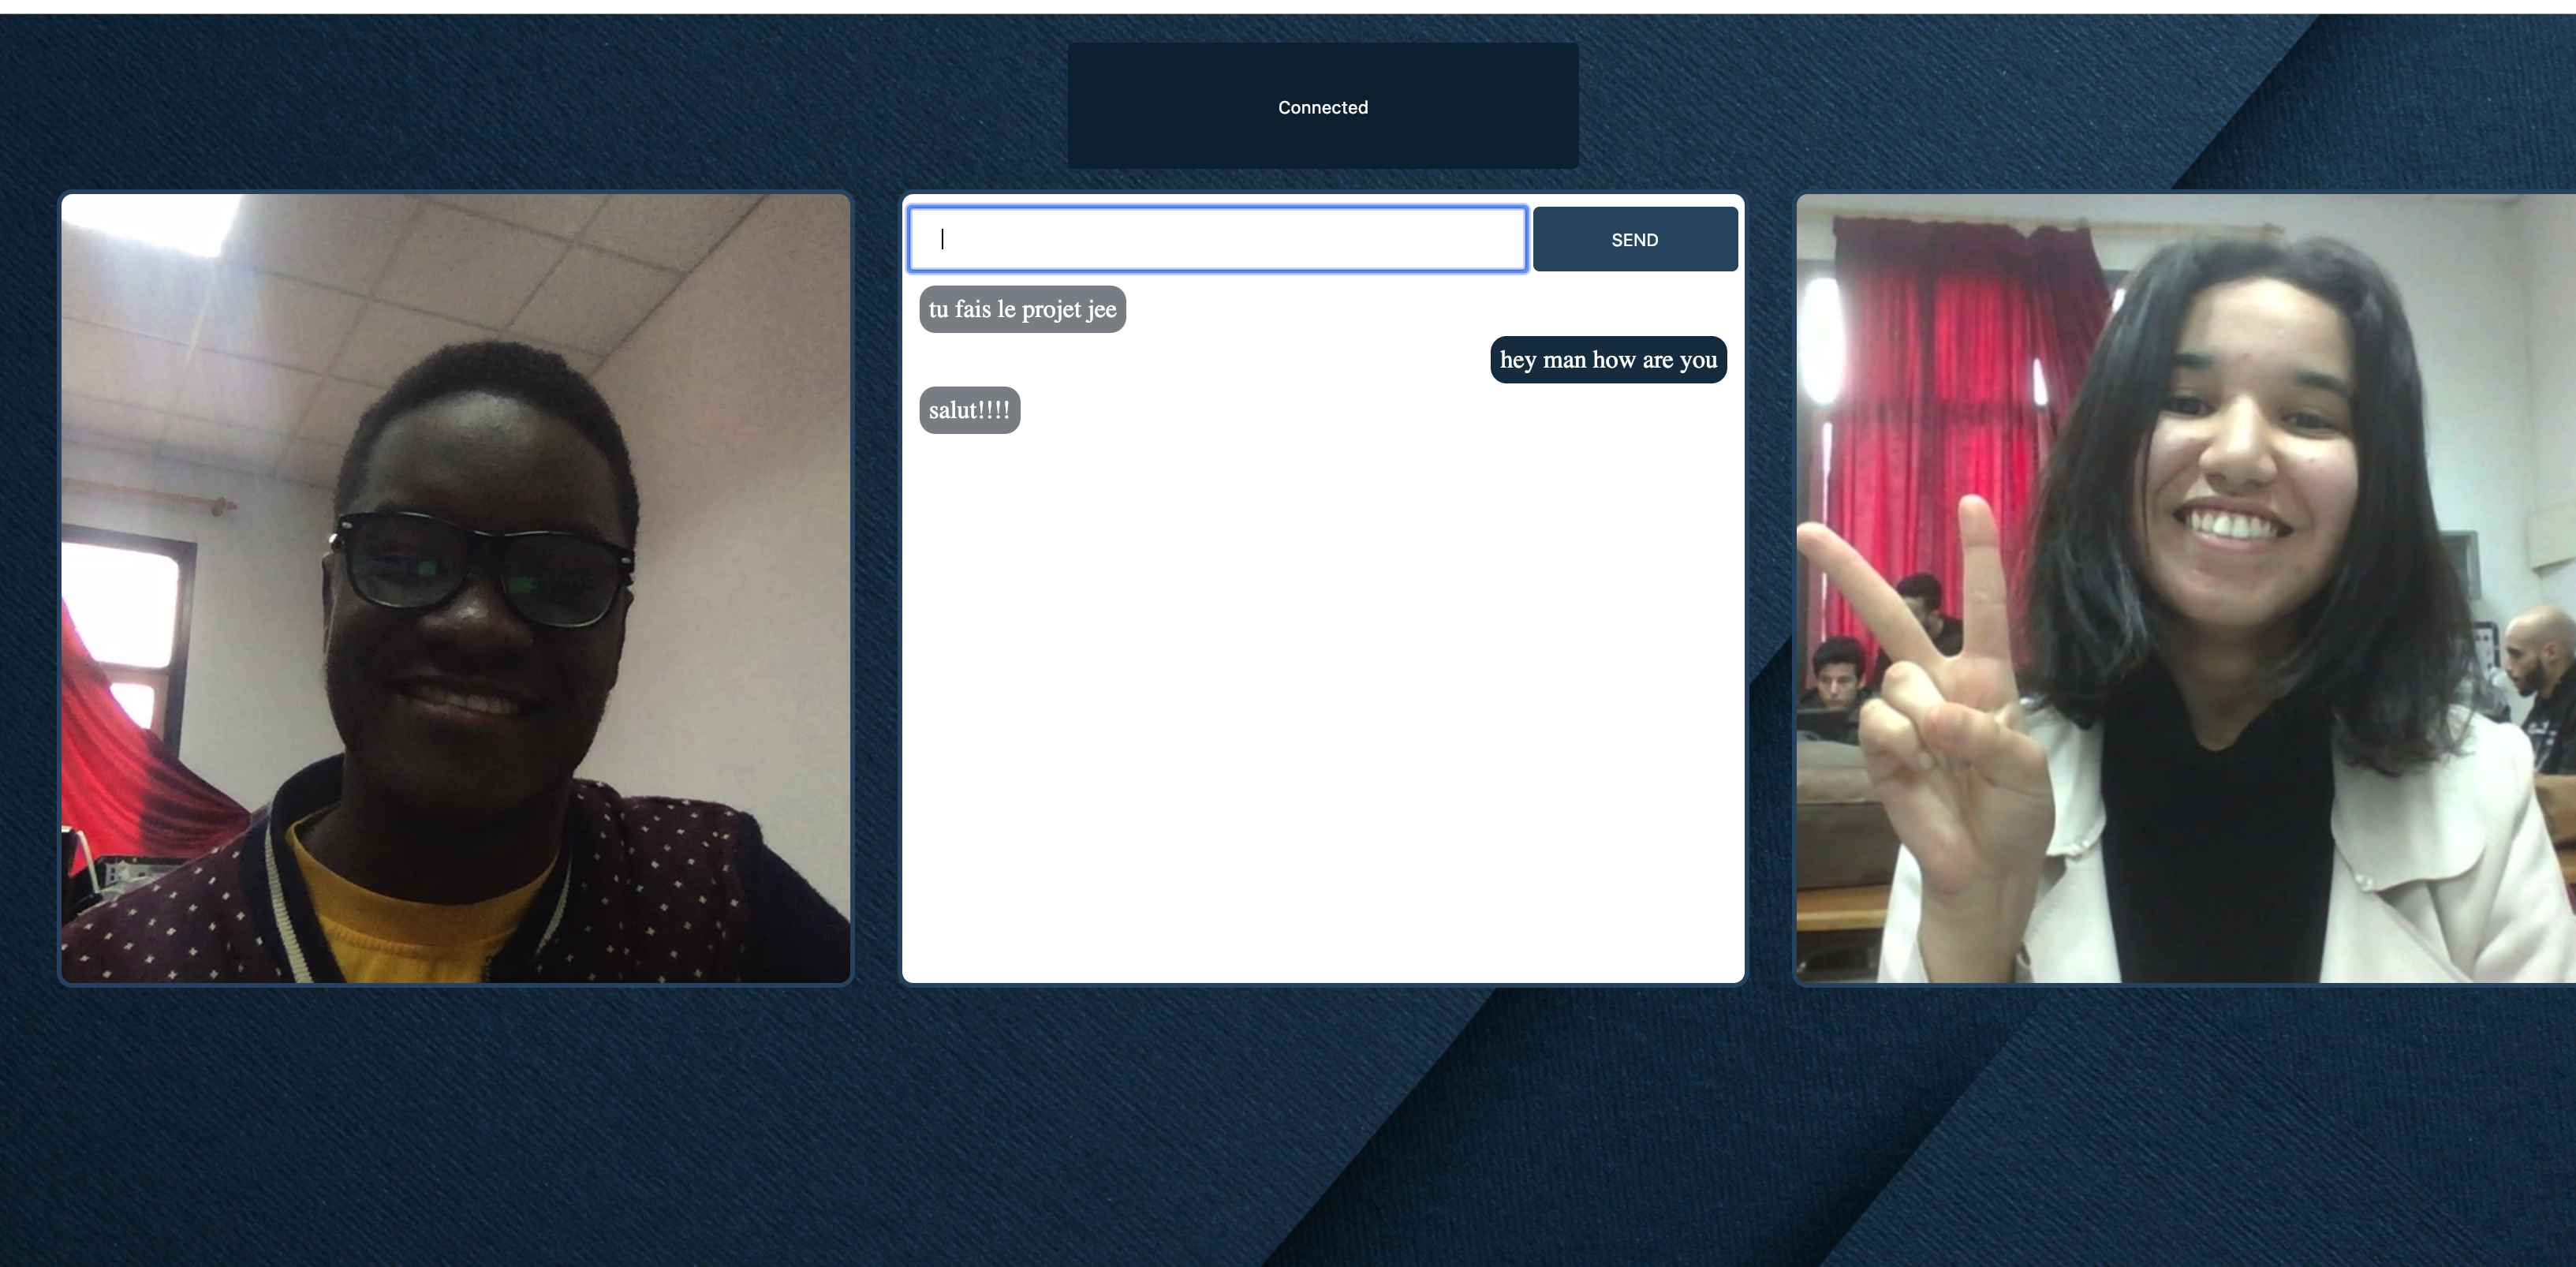
\includegraphics[width=.50\textwidth]{chatvideo.png}};
  \node[inner sep=0pt] (rapport) at (13,-3)
    { \\ \\ \\ \includegraphics[width=0.8\textwidth]{rapport.png}};
  
\node[align=center] at (13.5,-10) {
\\
\large 
Encadré par \textbf{
Professeur HAMLAOUI %%%% professeur %%%%
}\\ \\ \\ \large 
Préparée au sein de l'ENSIAS %%%% ÉCOLE  %%%%
 \large 
Filière : \textbf{
Génie Logiciel %%%% SPÉCIALITÉ %%%%
}\\ \\ \\ \\ \\ \large 
Présentée par : \textbf{
Amal Sahyani et TOURE Sidi %%%% NOM %%%%
}\\};
\node[draw, align=center] at (13.5,-17) {\, \hspace{12cm}
\\ \Large \textbf{ 
peer-to-peer VIDEOCHAT} \\ 
\\ \large \textbf{
projet jee %%%% SOUS-TITRE %%%%
}};
\node[align=center] at (13.5,-20) {Soutenue le
30/01/2019 %%%% DATE %%%%
};
//
//
//
//
\end{tikzpicture}
%%%%%%%%%%%%%%%%%%%%%%%%%%%%%%%%%%%%%%%%%%%%%%%%%%%%%%%%%%%%%
%%%%%%%%%%%%%%%%%%%%%%%%%%%%%%%%%%%%%%%%%%%%%%%%%%%%%%%%%%%%%


\newpage

\chapter*{Résumé}
\thispagestyle{empty}

Le sujet de notre projet de jee consistait à développer une « application de chatVideo en utilisant JEE ».Notre travail s’est fait en plusieurs phases: Une phase d’analyse et de conception et une phase de développement.
Grace à l’aide de notre encadrant, on a appris, au travers de ce prjet, à utiliser différents outils et découvert plusieurs concepts qui nous ont aidés à développer cette application.
on vous présentera donc tout au long de ce rapport, les étapes que nous avons suivis
ainsi que les outils que nous avons utilisés pour réaliser notre projet de JEE.
 %%%% INTÉGRER ICI LE RÉSUMÉ %%%%

\chapter*{Remerciements}
\thispagestyle{empty}

Au terme de ce travail, on profite de l’occasion pour remercier du fond du cœur tous ceux qui ont participé de près ou de loin à la réalisation de ce projet de jee et qui ont contribué à en faire une expérience enrichissante, on’adresse donc, en particulier mes sincères remerciements à notre encadrant Mr El HAMLAOUI pour sa disponibilité et ses précieux conseils.
\\
\\
Cordialement, Amal \& SIDI.%%%% INTÉGRER ICI LES REMERCIEMENTS %%%%

\renewcommand{\contentsname}{Sommaire}
\renewcommand\thepage{}
\tableofcontents
\thispagestyle{empty}

\mainmatter
\chapter*{Introduction}
\addcontentsline{toc}{chapter}{Introduction}
\chaptermark{Introduction}

%%%%%%%%%%%%%%%%%%%%%%%%%%%%%%%%%%%%%%%%%%%%%%%%%%%%%%%%%%
%%%%%%%%%%%%%%%%%%%%% Manuscrit %%%%%%%%%%%%%%%%%%%%%%%%%%


Ceci est une introduction

\chapter{Contexte général du projet}

intro du premier chapitre

\section{Problématique}



 AU deuxième trimestre 2018, Facebook annonça avoir plus de 2,27 milliards d'utilisateurs actifs chaque mois et 1,49 milliard d'utilisateurs actifs chaque jour dans le monde.cela ne laisse pas inapperçu l'attirance que les gens ont pour les réseaux sociaux. mais de nos jours, les réseaux sociaux se multiplie tellement que les gens se reservent soit pour des raisons de sécurité, soit par le fait qu'ils nous font perdre du temps sans pouvoir aller plus loin dans nos discussion. Ainsi, il sera question de trouver des moyens de communication plus fiable et avantageux que l'existants. 
Aussi pour permettre au personne de se rencontrer ayant chacun un motif et un profil différent, Une méthode de profils et des interêt des utilisateurs est essentielle pour de belles rencontre. Cette application servira donc à identifier, gérer et manipuler toutes ces informations correctement et avec plus de facilité.

\section{Bésoin et Solution}

Notre projet de JEE consiste donc à développer une application pour gérer les chats video entre des personnes ayant des interêts communs. \\
  L’objectif est de ne pas avoir à stocker les informations liées aux utilisateurs dans une base de données et de permettre à la classe métier de retrouver et de filtrer facilement les données ( tag et id) relative à chaque utilisateur dont il peut avoir besoin pour orienter et assurer la connexion entre eux. L’objectif sera également d’avoir une approche originale et différente par rapport au sujet et d’utiliser au mieux les outils dont nous disposons pour mettre au point ce projet.


\begin{figure*}[ht]
\centering\includegraphics[width=0.5\linewidth]{paulVa}
\caption{légende de la figure}
\end{figure*}


%%%exemple de citation de \cite{Sbirre1906}%%%

\bigskip

  


\chapter{Analyse et conception}
Ce chapitre abordera une analyse du sujet pour présenter une approche
originale et une modélisation de l’application.



\section{	Analyse et approche}
La majorité des applications de chat se contentent d’informations basiques et plutôt bornées relatives au profil, à la possibilité de communiquer et au traitement des publications, ainsi on y retrouve les identifiants et les motifs(tags) etc...Mais on y retrouve rarement des moyens de communiquer avec des inconnus pouvant avoir les même interêts que nous et acceptant de communiquer en video, avec des centres d’intérêts communs, gardant l’environnement ou l’entourage de l'utilisateur inconnu, ce qui pourtant serait d’une grande utilité pour la sécurité de l'utilisateur et de ses informations et pour découvrir ses attentes autant au niveau physique qu’au niveau vie dans le quotidien pour lui offrir le meilleur ,mieux l’encadrer et mieux l’orienter.\\
Et c’est donc grâce aux conseils de notre encadrant Mme El HAMLAOUI que on a décidé de suivre une approche différente et de nous éloigner du modèle basique des site de rencontre et de nous rapprocher du modèle où l’on traite ses centres d’intérêts, ses difficultés et ses choix pour lui donner le choix de choisir de quoi voudra t-il en parler tout en gardant ses information inconnues. les utilisateurs peuvent se faire des ateliers particuliers, des propositions de traitements qui lui conviennent ou de s'inviter à participer à des événements sportives, artistiques ou culturelles organisés par d'autres utilisateurs.
% \subsection{Titre de sous-partie}

\section{Modélisation}
 La modélisation du projet a été un point très important dans notre processus de travail vu qu’elle nous a permis d’aborder la structure de l’application et de mettre au point les objectifs à atteindre. Ainsi, pour une plus grande accessibilité de l’application nous avons opté pour un site web dynamique qui offrira une possibilité de connexion sans avoir à faire des identifications et qui offrira deux cas de figures :\\
•	L'accès à la page de connexion pour la génération d'un identifiant qui sera offert par la RTC pour
L'utilisateur qui une fois sur son compte pourra ecrire ses tags, soumettre les mots portant sur ces centres d’intérêts, son environnement etc.…et observer les personnes auxquels il a des interêts communs. 

\begin{figure*}[ht]
\centering\includegraphics[width=0.7\linewidth]{interaction.png}
\caption{Interaction Utilisateurs-system}
\end{figure*}
• La connexion grâce aux identifiants Administrateur-serveur pour les developpeurs ou pour le propriétaire qui une fois sur leurs comptes pourront filtrer les utilisateurs selon leurs tags et leurs centres d’intérêts pour leurs proposer de participer à des événements ou des opportunités de rencontre.

\begin{figure*}[ht]
\centering\includegraphics[width=0.7\linewidth]{administrateur.png}
\caption{Interaction administrateur-system}
\end{figure*}



\chapter{ Réalisation}
Ce chapitre abordera les outils que nous avons choisies d’utiliser, et présentera le résultat final de l’application.


\section{Outils de travail }
\subsection{Le langage HTML}
L’Hypertext Markup Language, généralement abrégé HTML, est le format de données conçu pour représenter les pages web. C’est un langage de balisage qui permet d’écrire de l’hypertexte, d’où son nom. HTML permet également de structurer sémantiquement et de mettre en forme le contenu des pages, d’inclure
des ressources multimédias dont des images et des formulaires de saisie.
On utilisera du CSS pour le colorage et formatages de ces textes.
\begin{figure*}[ht]
\centering\includegraphics[width=0.7\linewidth]{html.png}
\caption{image du langage html-css}
\end{figure*}

\subsection{Java EE}
Java Platform, Enterprise Edition, Java EE ou Jakarta EE (anciennement Java 2 Platform, Enterprise Edition, ou J2EE /ʒi.dø.ø.ø/1), est une spécification pour la plate-forme Java d'Oracle, destinée aux applications d'entreprise2.\\
La plate-forme étend Java Platform, Standard Edition (Java SE) en fournissant une API de mapping objet-relationnel, des architectures distribuées et multitiers, et des services web3. La plate-forme se fonde principalement sur des composants modulaires exécutés sur un serveur d'applications.
\begin{figure*}[ht]
\centering\includegraphics[width=0.7\linewidth]{Java_jee.png}
\caption{java jee }
\end{figure*}

\subsection{RTCweb}
\begin{figure*}[ht]
\centering\includegraphics[width=0.7\linewidth]{webrtc.png}
\caption{webrtc processus}
\end{figure*}
WebRTC (Web Real-Time Communication, littéralement « communication en temps réel pour le Web ») est une interface de programmation (API) JavaScript développée au sein du W3C et de l'IETF. C'est aussi un canevas logiciel avec des implémentations précoces dans différents navigateurs web pour permettre une communication en temps réel. Le but du WebRTC est de lier des applications comme la voix sur IP, le partage de fichiers en pair à pair en s'affranchissant des modules d'extensions propriétaires jusqu'alors nécessaires.
L'API repose sur une architecture triangulaire puis pair à pair dans laquelle un serveur central est utilisé pour mettre en relation deux pairs désirant échanger des flux de médias ou de données qui échangent ensuite sans autre relais. Cette architecture et la pile de protocoles utilisée posent des questions de sécurité et d'utilisation en relation avec d'autres technologies (comme les NAT ou les pare-feux) qui sont pour la plupart en cours de résolution par l'IETF et le W3C.

La technologie WebRTC étant assez récente, son intégration au sein des différents navigateurs est encore inégale ; bien que cela soit partiellement résolu par l'utilisation d'extensions propriétaires comme celle de Temasys1.
\begin{figure*}[ht]
\centering\includegraphics[width=0.7\linewidth]{webrtcbrowser.png}
\caption{webrtc browsers}
\end{figure*}


\subsection{Trello}
Trello est un outil de gestion de projet en ligne, lancé en septembre 2011, et inspiré par la méthode Kanban de Toyota. Il est basé sur une organisation des projets en planches listant des cartes, chacune représentant des tâches. Les cartes sont assignables à des utilisateurs et sont mobiles d'une planche à l'autre, traduisant leur avancement.

La version de base est gratuite, tandis qu'une formule payante permet d'obtenir des services supplémentaires. Le service est disponible en plusieurs langues (23 en juin 2016).

\begin{figure*}[ht]
\centering\includegraphics[width=0.7\linewidth]{trello.png}
\caption{trello logo}
\end{figure*}

\subsection{Share-Latex}
ShareLaTeX est un éditeur LaTeX en ligne, collaboratif, en temps réel et compileur PDF. Par ailleurs, ShareLaTeX fut libéré en février 20143. Le 20 Juillet 2017, ShareLatex a été racheté par Overleaf4 qui prévoit de réunir les services d'Overleaf et de Sharelatex sur une seule plateforme, actuellement en période de test5. La fusion des deux services au sein de Overleaf v2 est prévue pour le 4 septembre 20186.

En comparaison avec les autres éditeurs LaTeX, ShareLaTeX est une application basée sur un serveur web, qui est donc accessible via un navigateur internet. Une version publique, et maintenue, est disponible sur https://www.sharelatex.com [archive]. Les dépôts nécessaires à la création d'une instance personnelle de ShareLaTeX sont disponibles sous la licence AGPL v32.
\begin{figure*}[ht]
\centering\includegraphics[width=0.7\linewidth]{sharelatex.png}
\caption{sharelatex}
\end{figure*}
\section{Encore un titre original}

\section{Réalisation de l’application }
•page d'accueil
pas de Création de la base de données\\
Les informations receuillies grace aux tags donnés par l'utilisateur lors de son inscription impliquaient la présence d'un ensemble d'information sur le serveur pour les stocker et les traiter.Ainsi il fallait créer la base de données gestion utilisateurs aen utilisant le RMI.\\

\subsection{Création des pages Web}
La page d’accueil se doit d’être attractive et de présenter différentes fonctionnalités pour attirer le regard et l’intérêt des internautes, le titre du site se doit aussi d’être original pour les mêmes raisons.  Ainsi on a choisi une interface et des couleurs conviviales, ainsi qu’un titre « chatVideo» et un slogan « on va chatter en video ici » qui pousse à rester découvrir toutes les fonctionnalités du site.On peut accéder à différentes rubriques tel que « ajouter des tags » ou « A propos de l’Ensias » ou « Contactez nous »
\begin{figure*}[ht]
\centering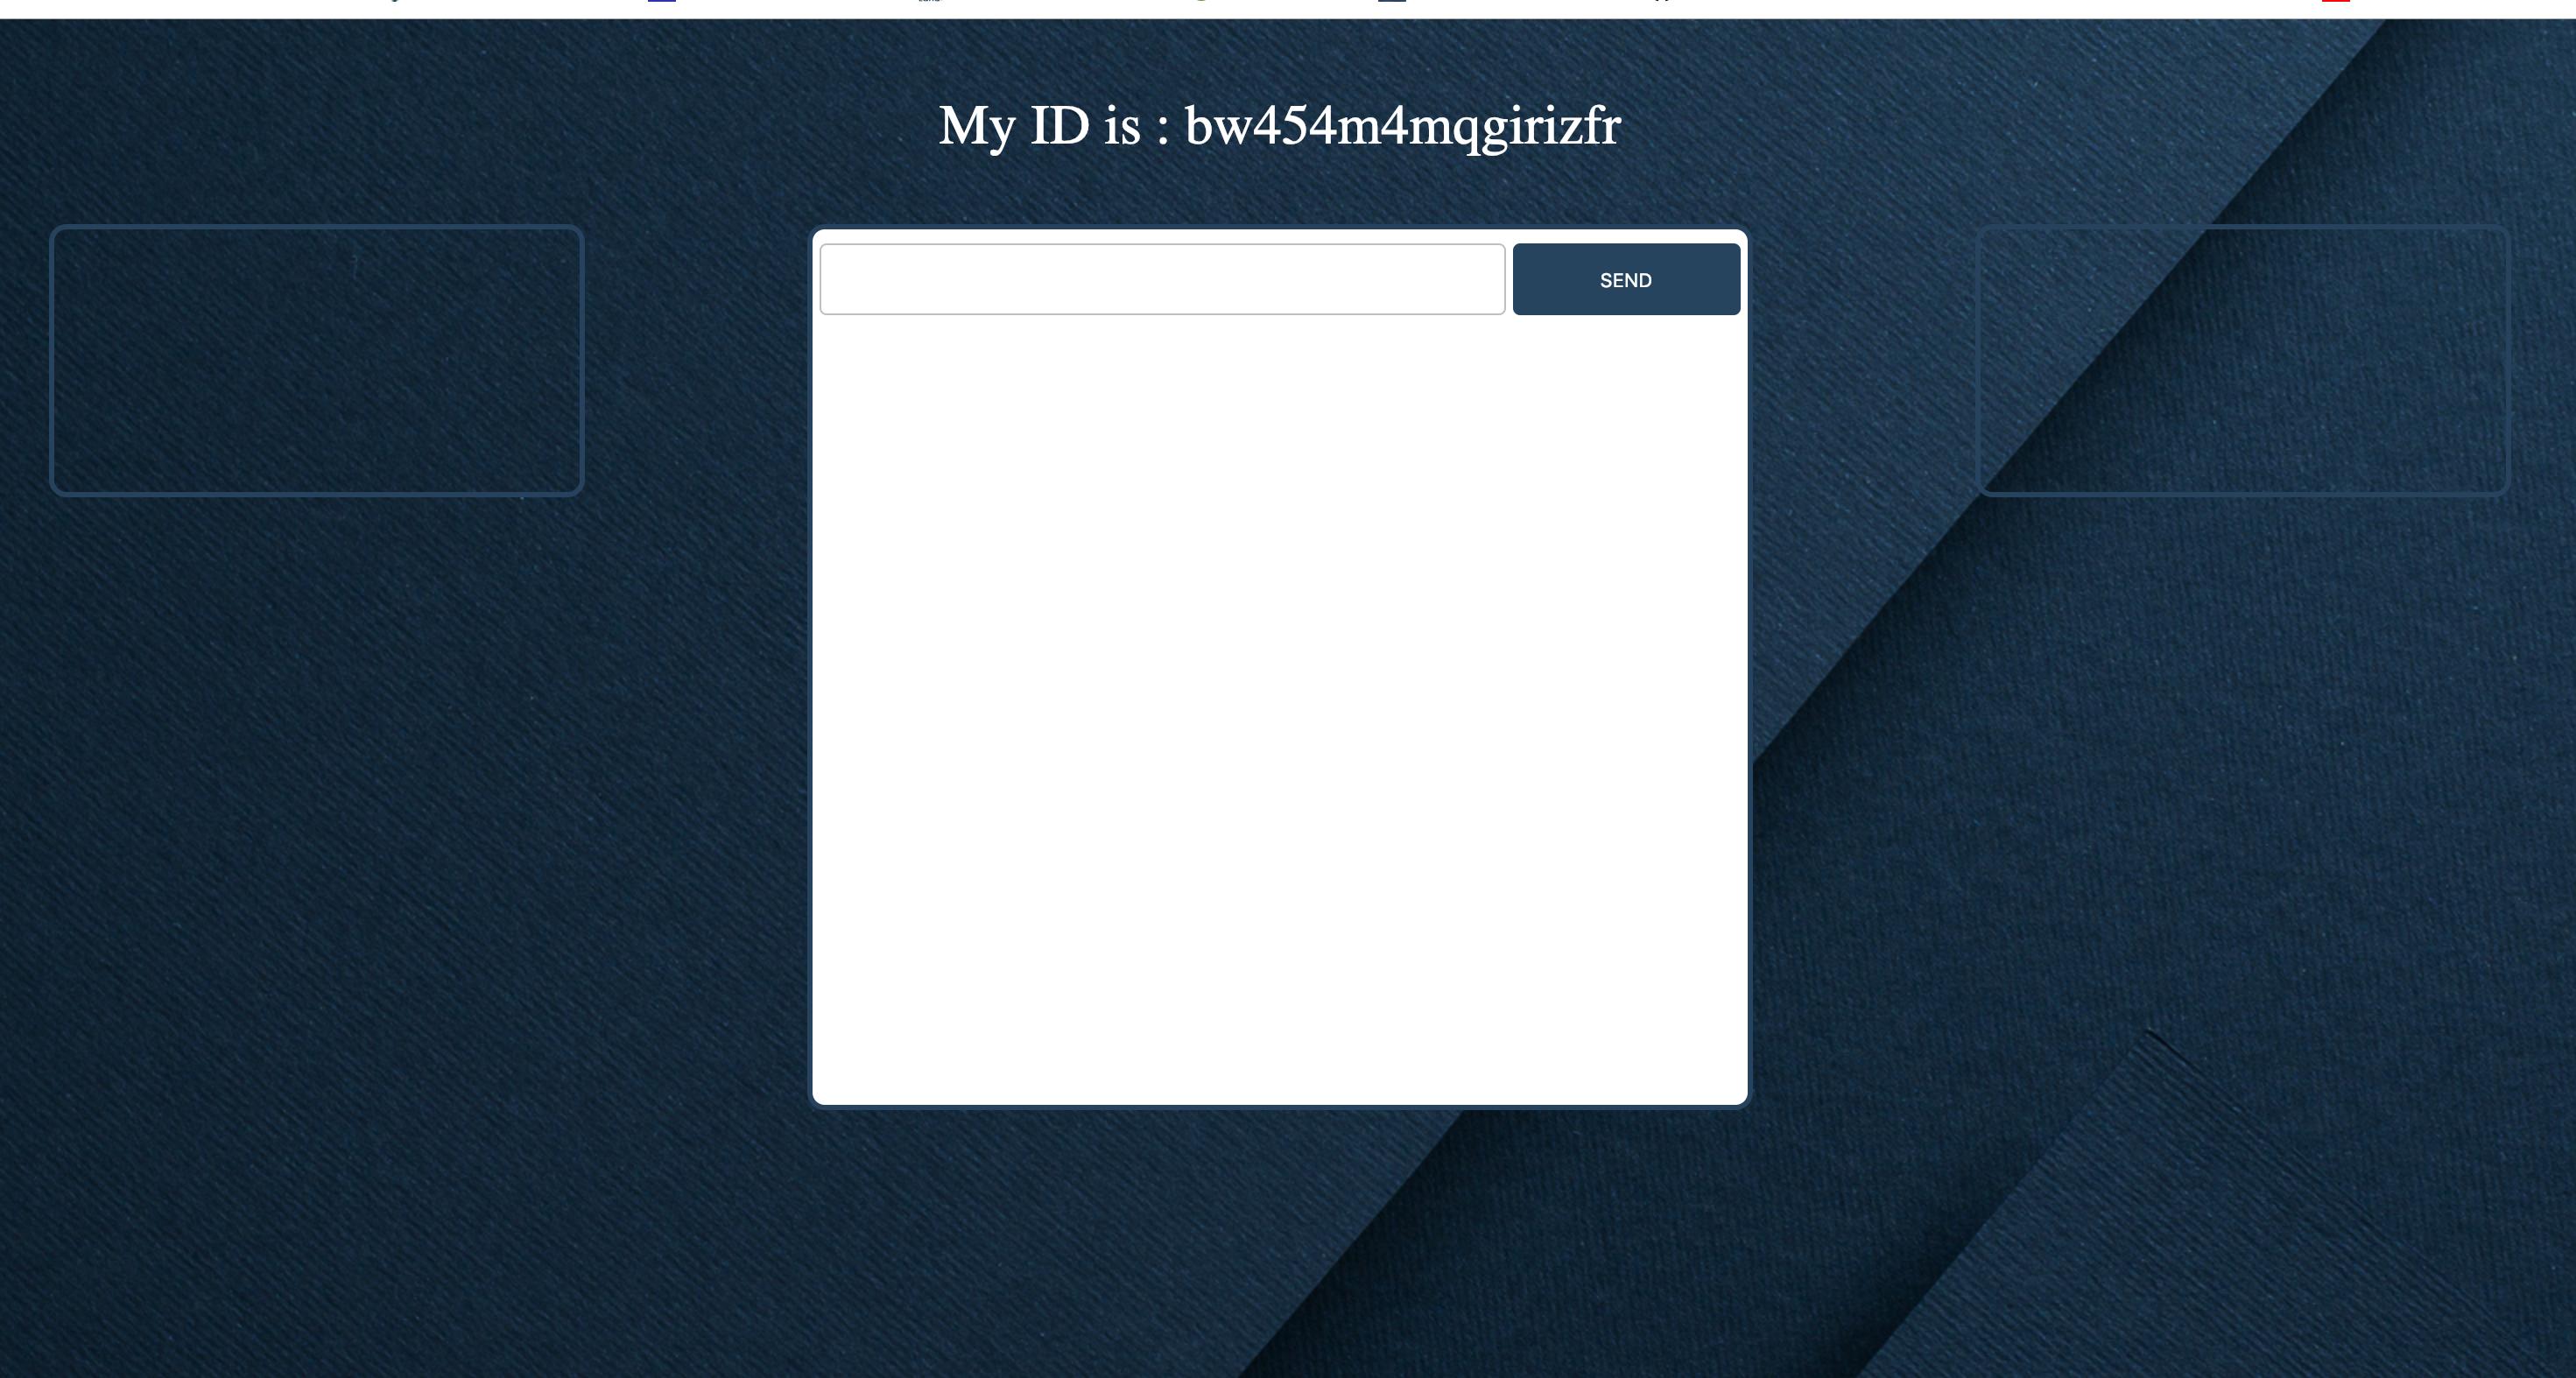
\includegraphics[width=0.7\linewidth]{accueil.png}
\caption{page d'accueil}
\end{figure*}
\\
•les tags\\
l'utilisateur doit pouvoir donner les tags concernant ses centres d'interêt
•connexion et génération d'id. \\
une fois que l'utilisateur arrive à sagir le tag, il aura besoin d'un id qui lui permettra d'être identifier par le webrtc. cet id sera stocker dans le serveur rmi tantqu'il ne trouvera un lautre user à qui se connecter.\\
•chat\\
Après connection, l'utilisateur doit pouvoir ecrire des messages à un autre, lire des audio et se voir en même temps.\\

\subsection{Gestion des erreurs :}
Pour éviter que les utilisateurs ne saisissent des messages vulgaires ou inappropriées et pour avoir des résultats cohérents au niveau des methodes de recherche pour les tags. il faut mettre en place un procédé de gestion d’erreurs .Pour cela les messages et reponses au aux questions du formulaire de tags sont sous forme de liste à remplir et dont certains mots ne seront pas acceptés. Au niveau du profil afin que la date de naissance soit sous format acceptable sous SQL on a mis au point une méthode avec une class java permettant une saisie correcte des tags.

\chapter{ Conclusion}
En substance, ce projet de JEE consistait à développer une application de chatVideo entre inconnu d'une manière aléatoire et avec des des tags. Je vous ai présenté tout au long de ce rapport la démarche que nous avons suivie pour mettre au point cette application. Toute fois pour améliorer notre application on peut développer la section suggestions pour que les utilisateurs reçoivent quotidiennement des propositions d’événement ou de rencontres grâce à une messagerie interne en collectant uniquement le mail et les centres d'interêt de la personne. Comme on peut pour un profil plus complet de l’utilisateur, ajouter une gestion de rencoontre suivants les tags et ces activités.\\
Ce projet de j2e a été une belle occasion pour travailler sur une application de chat, pour développer nos connaissances et nos compétences et surtout pour découvrir de nouvelles fonctionnalités à l’instar de « J2E », « WebRTC » et de langages tel que « js» « html/css ».



\newpage
\addcontentsline{toc}{chapter}{Bibliographie}
\pagestyle{plain}
lien git: https://github.com/ENSIAS-MEH/JEE2019_Groupe1-4.git \\
lien: shareLatex: https://www.overleaf.com/project/5c50a229d34a0e784f263f30 \\
\thispagestyle{plain}
\pagestyle{fancy}

\appendix
\chapter{Première annexe}
\pagenumbering{Roman}
\setcounter{page}{1}

Ceci est en annexe

\end{document}
